\documentclass{beamer}
\usepackage{array}
\usepackage{graphicx}
\usepackage{german}
%\usepackage{txfonts}

\mode<beamer>{%
\usetheme[hideothersubsections,hidetitle]{Hannover}
}
\title[]{Partielle Differentialgleichungen}
\subtitle{3. Sitzung: Separation}
\date[9.~M"arz 2016]{9.~M"arz 2016}
\author{Prof.~Dr.~Andreas M"uller}
\begin{document}

\begin{frame}
\titlepage
\end{frame}

\begin{frame}
\frametitle{Idee}
{\bf Voraussetzung:}
$F(x)$ und $G(y)$ Funktionen nur einer Variable mit
\[
F(x)=G(y)
\]
\pause
{\bf Folgerung:} beide konstant
\begin{align*}
F(x)&=\color{red}\mu\\
G(y)&=\color{red}\mu
\end{align*}
\pause
{\bf Gewinn:}
\begin{enumerate}
\item Zwei Gleichungen mit je {\bf nur einer Variablen}
\item Preis: eine zus"atzliche Unbekannte $\color{red}\mu$
\end{enumerate}
\pause
Achtung: L"osungen f"ur verschiedene $\mu$ m"oglich
\end{frame}

\begin{frame}
\frametitle{Differentialgleichungen}
{\bf Differentialgleichung:}
\[
F\biggl(x, y, u,
\frac{\partial u}{\partial x},
\frac{\partial u}{\partial y},\dots\biggr)=0
\]
\pause
{\bf Ansatz:}
\begin{align*}
&\text{meistens:}&
u(x,y)&=X(x)\cdot Y(y)\\
&\text{manchmal:}&
u(x,y)&=X(x) + Y(y)
\end{align*}
\pause
{\bf Einsetzen:}
\[
\text{Terme mit $x$} = \text{Terme mit $y$}
\]
\pause
{\bf Separation:}
\begin{align*}
\text{Differentialgleichung in $x$}&= \color{red}\mu\\
\text{Differentialgleichung in $y$}&= \color{red}\mu
\end{align*}
\end{frame}

\begin{frame}
\frametitle{Schwingende Saite}
{\bf Differentialgleichung:}
\[
\frac{\partial^2 u}{\partial t^2}
=
\frac{\partial^2 u}{\partial x^2}
\]
{\bf Gebiet:}
\[
\Omega = \{ (t,x) \,|\, t>0, 0<x<\pi\}
\]
{\bf Randbedingungen:}
\begin{align*}
u(t,0)&=u(t,\pi)=0\\
u(0,x)&=f(x)&\frac{\partial u}{\partial t}(0,x)&=g(x)
\end{align*}
\begin{enumerate}
\pause
\item Separationsansatz
\item Einsetzen
\item Separieren
\item Teilgleichung l"osen
\end{enumerate}
\end{frame}

\begin{frame}
\frametitle{Schwingende Saite}
\begin{center}
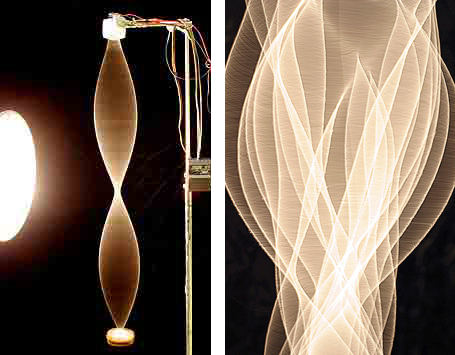
\includegraphics[width=\hsize]{../../skript/graphics/stringvibrlarge-10-06-06.jpg}
\end{center}
\end{frame}

\begin{frame}
\frametitle{Eigenwertproblem}
Partielle Differentialgleichung:
\[
\frac{\partial^2 u}{\partial t^2}
=
\frac{\partial^2 u}{\partial x^2}
\]
Separation mit Ansatz $u(t,x)=T(t)X(x)$:
\begin{align*}
T''(t)&=\lambda T(t)
&
X''(x)&=\lambda X(x)
\end{align*}
\pause
Eigenwertproblem: Finde $\color{red} X$ und $\color{red}\lambda$ so,
dass
\[
{\color{red} X}''(x)={\color{red}\lambda} {\color{red} X}(x)
\]
$\Rightarrow$
\pause
\begin{enumerate}
\item
nicht jeder Wert $\lambda$ ist m"oglich
\pause
\item
Randbedingungen legen m"ogliche Werte fest
\end{enumerate}
\end{frame}

\begin{frame}
\frametitle{"Uberlagerungsprinzip}
Wenn
$u_n(x,y)$
L"osungen der Differentialgleichung sind
\pause
\[
\Rightarrow
\quad
u(x,y)=\sum_{n}a_nu_n(x,y)
\]
ist auch eine L"osung.

\medskip
\pause
Zwei Arten von Randbedingungen:
\begin{itemize}
\item Nullbedingungen: schr"ankt $u_n$ ein
\item restliche Bedingungen: Bestimmung von $a_n$
\end{itemize}
\end{frame}

\begin{frame}
\frametitle{Zusammenfassung: Separation}
\begin{enumerate}
\item Koordinaten: m"ussen zu Gebietsgrenzen passen
\pause
\item Separationsansatz: 
\begin{align*}
&\text{meistens:}&u(x,y)&=X(x)\cdot Y(y)\\
&\text{manchmal:}&u(x,y)&=X(x)+Y(y)
\end{align*}
\pause
\item Einsetzen und Variablen trennen
\[
\text{nur $x$} = \text{nur y}\quad\Rightarrow\quad \text{beide konstant $=\mu$}
\]
$\Rightarrow$ Eigenwertproblem
\pause
\item Nullrandbedingungen legen $\mu$ fest: $\mu_1$, $\mu_2$,
$\mu_3,\dots,\mu_n,\dots$
\pause
\item Teill"osungen $u_n(x,y)=X_n(x)\cdot Y_n(y)$  zu jedem $\mu_n$
\pause
\item "Uberlagerung (nur f"ur lineare PDGL)
\[
u(x,y)=\sum_n a_nu_n(x,y)
\]
\pause
\item Koeffizienten $a_n$ aus verbleibenden Randbedingungen
\end{enumerate}
\end{frame}

\end{document}
